\documentclass[varwidth,border=0pt]{standalone}

% Tikz packages
\usepackage{tikz}
\usetikzlibrary{%
  patterns, plotmarks, backgrounds, shapes, arrows, calc, trees, positioning,
  chains, shapes.geometric, decorations.pathreplacing,
  decorations.pathmorphing, shapes.arrows, decorations.markings, quotes,
  arrows.meta, spy, fit, matrix
}

% General image and colour support
\usepackage{graphicx}
\usepackage{xcolor}

% Captions and subcaptions
\usepackage{caption}
\usepackage[labelformat=parens]{subcaption}
\renewcommand\thesubfigure{\alph{subfigure})}

% Define main node type for networks
\tikzstyle{lnode} = [%
  circle,
  draw=black,
  minimum height=0.65cm,
  align=center,
  fill=none,
  text centered,
  inner sep=0.5pt,
  font=\tiny
]%

\begin{document}
  \vspace*{-1.0em}
  \begin{figure}
    \centering
    \begin{subfigure}[t]{0.5\textwidth}
      \caption{}
      \vspace*{-1.2em}
      \scalebox{0.70}{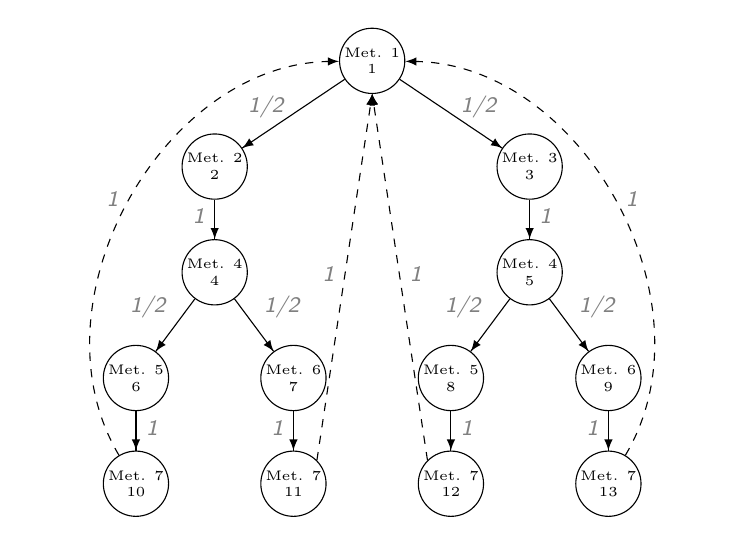
\begin{tikzpicture}[%
  >=latex,
  decoration={%
    markings,
    mark=at position 1.0 with {\arrow{>}}
  },
  every node/.style={%
    font=\sffamily\footnotesize\itshape,
    text=gray,
    text centered,
    align=center
  },
  frame/.style={draw=black,inner sep=2pt}
]

  % Nodes
  \node[lnode,text=black] (A1) {Met. 1\\1};
  \node[lnode,text=black,below=0.5cm of A1,xshift=-2.0cm] (A2) {Met. 2\\2};
  \node[lnode,text=black,below=0.5cm of A1,xshift=+2.0cm] (A3) {Met. 3\\3};
  \node[lnode,text=black,below=0.5cm of A2] (A42) {Met. 4\\4};
  \node[lnode,text=black,below=0.5cm of A3] (A43) {Met. 4\\5};
  \node[lnode,text=black,below=0.5cm of A42,xshift=-1.0cm] (A52) {Met. 5\\6};
  \node[lnode,text=black,below=0.5cm of A42,xshift=+1.0cm] (A62) {Met. 6\\7};
  \node[lnode,text=black,below=0.5cm of A43,xshift=-1.0cm] (A53) {Met. 5\\8};
  \node[lnode,text=black,below=0.5cm of A43,xshift=+1.0cm] (A63) {Met. 6\\9};
  \node[lnode,text=black,below=0.5cm of A52] (A752) {Met. 7\\10};
  \node[lnode,text=black,below=0.5cm of A62] (A762) {Met. 7\\11};
  \node[lnode,text=black,below=0.5cm of A53] (A753) {Met. 7\\12};
  \node[lnode,text=black,below=0.5cm of A63] (A763) {Met. 7\\13};

  % Intra-node edges
  \draw[postaction={decorate}] (A1) to node [above left=0.1pt,yshift=-5pt] {1/2} (A2);
  \draw[postaction={decorate}] (A1) to node [above right=0.1pt,yshift=-5pt] {1/2} (A3);
  \draw[postaction={decorate}] (A2) to node [left=0.1pt,yshift=+1pt] {1} (A42);
  \draw[postaction={decorate}] (A42) to node [above left=0.1pt,yshift=-1pt] {1/2} (A52);
  \draw[postaction={decorate}] (A42) to node [above right=0.1pt,yshift=-1pt] {1/2} (A62);
  \draw[postaction={decorate}] (A52) to node [right=0.1pt,yshift=+1pt] {1} (A752);
  \draw[postaction={decorate}] (A62) to node [left=0.1pt,yshift=+1pt] {1} (A762);
  \draw[postaction={decorate}] (A3) to node [right=0.1pt,yshift=+1pt] {1} (A43);
  \draw[postaction={decorate}] (A43) to node [above left=0.1pt,yshift=-1pt] {1/2} (A53);
  \draw[postaction={decorate}] (A43) to node [above right=0.1pt,yshift=-1pt] {1/2} (A63);
  \draw[postaction={decorate}] (A53) to node [right=0.1pt,yshift=+1pt] {1} (A753);
  \draw[postaction={decorate}] (A63) to node [left=0.1pt,yshift=+1pt] {1} (A763);

  % Boundary edges
  \draw[dashed,->, postaction={decorate}, bend left=60, distance=2.25cm] (A752) to node [left=0.1pt,yshift=+1pt] {1} (A1);
  \draw[dashed,->, postaction={decorate}] (A762.north east) to node [left=0.1pt,yshift=+1pt] {1} (A1.south);

  \draw[dashed,->, postaction={decorate}, bend right=60, distance=2.25cm] (A763) to node [right=0.1pt,yshift=+1pt] {1} (A1);
  \draw[dashed,->, postaction={decorate}] (A753.north west) to node [right=0.1pt,yshift=+1pt] {1} (A1.south);
  %\draw[->, postaction={decorate}, bend left=72, distance=2.0cm] (A7.south) to node [above=0.1pt,yshift=-3pt] {4} (A1.south);

\end{tikzpicture}

}
    \end{subfigure}\hfill%
    \begin{subfigure}[t]{0.5\textwidth}
      \caption{}
      \vspace*{-1.2em}
      \scalebox{0.70}{\input{input-example-2-cyclehistory.tex}}
    \end{subfigure}
  \end{figure}
\end{document}

